\documentclass[]{article}
\usepackage{lmodern}
\usepackage{amssymb,amsmath}
\usepackage{ifxetex,ifluatex}
\usepackage{fixltx2e} % provides \textsubscript
\ifnum 0\ifxetex 1\fi\ifluatex 1\fi=0 % if pdftex
  \usepackage[T1]{fontenc}
  \usepackage[utf8]{inputenc}
\else % if luatex or xelatex
  \ifxetex
    \usepackage{mathspec}
  \else
    \usepackage{fontspec}
  \fi
  \defaultfontfeatures{Ligatures=TeX,Scale=MatchLowercase}
\fi
% use upquote if available, for straight quotes in verbatim environments
\IfFileExists{upquote.sty}{\usepackage{upquote}}{}
% use microtype if available
\IfFileExists{microtype.sty}{%
\usepackage{microtype}
\UseMicrotypeSet[protrusion]{basicmath} % disable protrusion for tt fonts
}{}
\usepackage[unicode=true]{hyperref}
\hypersetup{
            pdfborder={0 0 0},
            breaklinks=true}
\urlstyle{same}  % don't use monospace font for urls
\usepackage{graphicx,grffile}
\makeatletter
\def\maxwidth{\ifdim\Gin@nat@width>\linewidth\linewidth\else\Gin@nat@width\fi}
\def\maxheight{\ifdim\Gin@nat@height>\textheight\textheight\else\Gin@nat@height\fi}
\makeatother
% Scale images if necessary, so that they will not overflow the page
% margins by default, and it is still possible to overwrite the defaults
% using explicit options in \includegraphics[width, height, ...]{}
\setkeys{Gin}{width=\maxwidth,height=\maxheight,keepaspectratio}
\IfFileExists{parskip.sty}{%
\usepackage{parskip}
}{% else
\setlength{\parindent}{0pt}
\setlength{\parskip}{6pt plus 2pt minus 1pt}
}
\setlength{\emergencystretch}{3em}  % prevent overfull lines
\providecommand{\tightlist}{%
  \setlength{\itemsep}{0pt}\setlength{\parskip}{0pt}}
\setcounter{secnumdepth}{0}
% Redefines (sub)paragraphs to behave more like sections
\ifx\paragraph\undefined\else
\let\oldparagraph\paragraph
\renewcommand{\paragraph}[1]{\oldparagraph{#1}\mbox{}}
\fi
\ifx\subparagraph\undefined\else
\let\oldsubparagraph\subparagraph
\renewcommand{\subparagraph}[1]{\oldsubparagraph{#1}\mbox{}}
\fi

% set default figure placement to htbp
\makeatletter
\def\fps@figure{htbp}
\makeatother


\date{}

\begin{document}

\begin{quote}
\textbf{\emph{TERAPIA FISICA}}
\end{quote}

I mezzi fisici sono stati utilizzati perché si ritiene abbiano effetti
biologici, anche se per alcuni mezzi fisici gli effetti biologici
presupposti non sono stati interamente dimostrati, ad esempio nel caso
degli ultrasuoni, utilizzati da oltre 25 anni senza alcuna spiegazione
scientifica del loro effetto.

\begin{quote}
\textbf{\emph{TERMOTERAPIA}}
\end{quote}

Il calore ha effetti locali, riflessi (a distanza), determina
un'accelerazione dei processi metabolici ed una stimolazione delle fibre
nervose sensitive.

\begin{quote}
Si divide in: - \textbf{TERMOTERAPIA ENDOGENA:} il calore si produce in
profondità all'interno del

tessuto che stiamo trattando,

- \textbf{TERMOTERAPIA ESOGENA:} produce calore direttamente sul
tessuto, in quanto il mezzo

fisico che noi utilizziamo si scalda (sabbia, fanghi, paraffina, bagni
termali, bagno turco, sauna, la doccia).

I mezzi fisici utilizzati per la termoterapia endogena sono
rappresentati dalla \textbf{corrente elettrica}, \textbf{radiazioni
elettromagnetiche, ultrasuoni} (a metà tra esogena ed endogena, perché
la testina che li produce si scalda ma produce calore in profondità).
\end{quote}

Le applicazioni di termoterapia variano dai 15 ai 30 minuti, in cicli di
10 applicazioni quotidiane (numero comune a tutti i mezzi fisici).

\begin{quote}
\textbf{Indicazioni}
\end{quote}

Artropatie croniche (non acute, che sono controindicate): lombalgie,
gonartrosi, osteocondrosi. Possiamo utilizzarla come preparazione
all'applicazione di kinesiterapie.

\textbf{Controindicazioni generali}, ovvero comuni a tutti i mezzi
fisici, sono gravidanza, tumori, flogosi; le controindicazioni
specifiche della termoterapia riguardano la pressione arteriosa del
paziente, disturbi cardiovascolari, trombosi, flebiti, tromboflebiti,
diabete (pazienti con neuropatia periferica potrebbero non percepire
correttamente l'entità dello stimolo applicato, potendo arrivare a
subire ustioni).

La paraffinoterapia è stata spesso utilizzata in passato, ora è rara,
perché è complicata la sua utilizzazione ed i centri riabilitativi
abilitati sono pochi.

\begin{quote}
\textbf{\emph{ELETTROTERAPIA}}

Classificazione dell'elettroterapia: - \textbf{direzione della corrente}
(unidirezionale o bidirezionale),

- \textbf{intensità della corrente} (continua o variabile).

Queste correnti possono avere \textbf{azioni} diverse, che vanno da
quella \textbf{antalgica} a quella \textbf{trofica} o

\textbf{eccitomotoria}.
\end{quote}

Le correnti maggiormente utilizzate in riabilitazione sono di tipo
\emph{variabile unidirezionale}, che rientrano nell'ambito delle
correnti \emph{antalgiche}.

Le correnti \emph{variabili bidirezionali} invece possono essere a bassa
o media frequenza, con scopo analgesico per la bassa frequenza o
eccitomotorio per la media frequenza.

Le correnti \textbf{variabili} vengono utilizzate per stimolare un
muscolo che può essere normalmente innervato oppure parzialmente o
totalmente denervato. C'è una differenza perché a seconda se si dovrà
stimolare una cellula muscolare o nervosa bisognerà applicare uno
stimolo elettrico più o meno lungo.

Quando si applica un \textbf{impulso elettrico} questo dovrà essere
tollerato dal paziente, perciò si andrà in base alla

\textbf{soglia} del paziente, che dovrà percepire l'impulso senza però
avvertirlo come fastidioso o intollerabile.

\begin{quote}
Le \textbf{caratteristiche di un impulso} sono l'ampiezza, la durata, il
tempo di salita e di discesa, la pausa tra gli impulsi (il doppio della
durata).
\end{quote}

L'impulso può essere di \textbf{forma: - rettangolare}: sono
eccitomotori per muscoli normalmente innervati,

\begin{itemize}
\item
  \textbf{triangolare}: agiscono su muscoli parzialmente o totalmente
  denervati (hanno breve durata),
\item
  \begin{quote}
  \textbf{esponenziale}: come sopra
  \end{quote}
\item
  \begin{quote}
  \textbf{quadrata}: hanno effetto antalgico
  \end{quote}
\end{itemize}

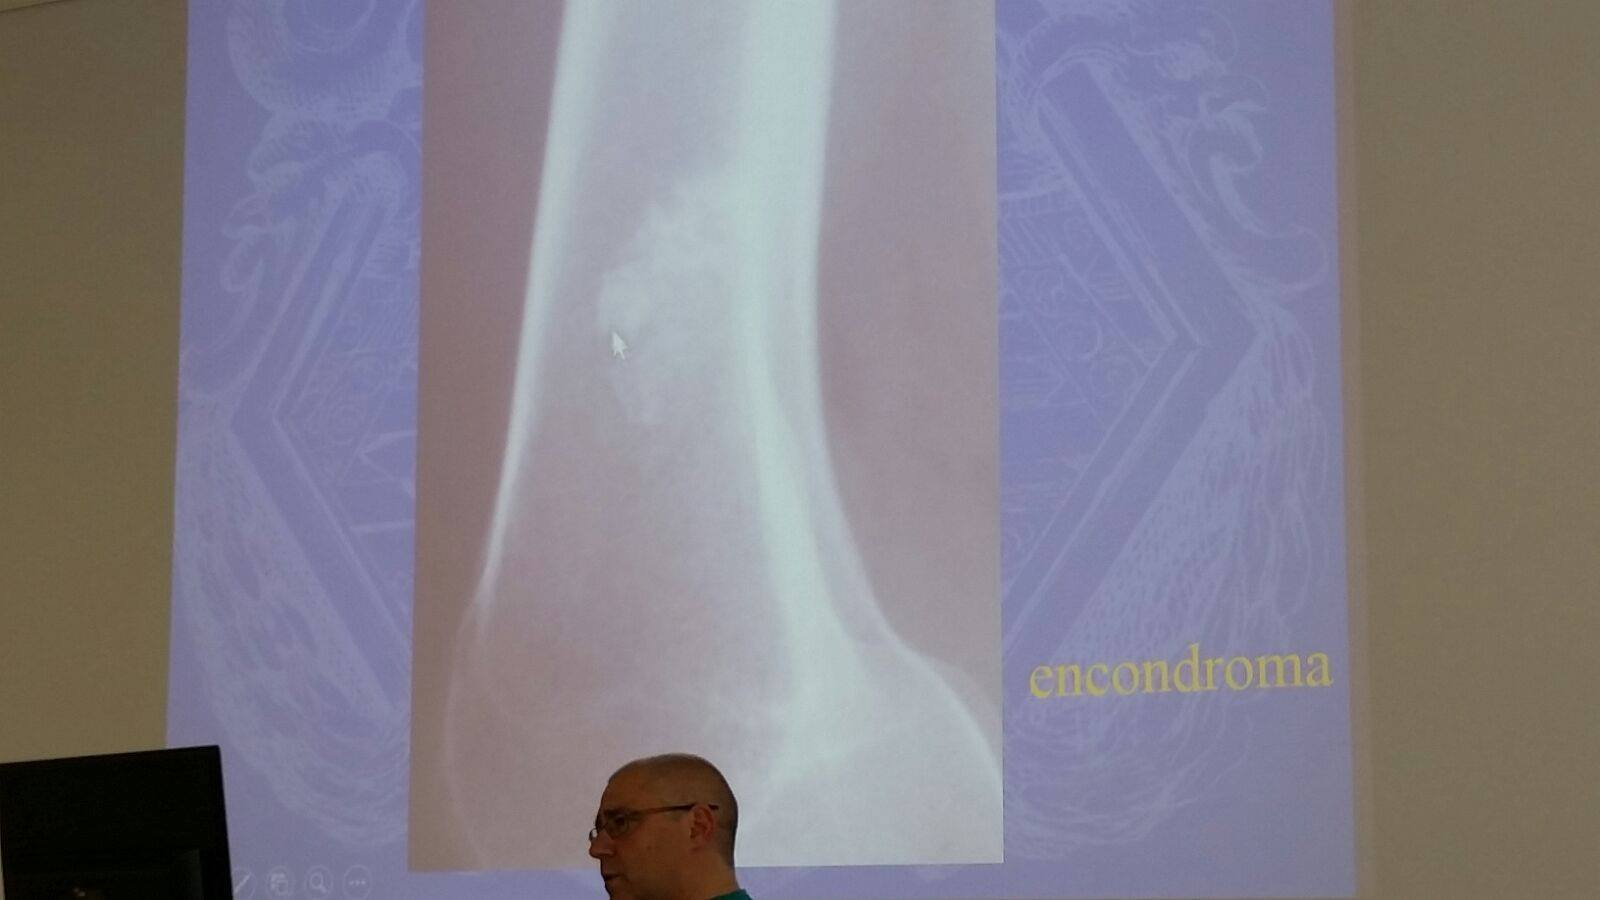
\includegraphics[width=6.64653in,height=6.08472in]{media/image1.jpeg}

\begin{quote}
\textbf{Dal punto di vista terapeutico} l'elettroterapia può essere
suddivisa in:
\end{quote}

\begin{itemize}
\item
  terapia di stimolazione,
\item
  correnti che veicolano farmaci (ionoforesi, utilizzata in passato),
\item
  terapia antalgica (TENS e correnti diadinamiche).
\end{itemize}

Qualsiasi forma di corrente elettrica applicata localmente deve
\textbf{rispettare alcuni criteri}: la cute deve essere ben detersa,
senza peli, integra; si applicano elettrodi con l'interposizione di un
gel conduttivo; la corrente deve essere percepita dal paziente, come
detto prima; fare attenzione al fenomeno dell'accomodazione: ad ogni
impulso applicato la soglia del paziente si alzerà, perciò si dovrà
leggermente innalzare l'intensità degli impulsi;

Le correnti \emph{rettangolari della \textbf{terapia di STIMOLAZIONE
}}vanno applicate con precisione; ogni uscita del macchinario ha due
elettrodi: rosso positivo e nero negativo. Il negativo va applicato
sull'estremità opposta del muscolo, mentre il positivo direttamente sul
ventre muscolare laddove pensiamo possa esserci la placca motrice. La
durata media di applicazione va dai 20 ai 30 minuti.

Per quanto riguarda \textbf{l'elettroterapia antalgica} abbiamo la
\textbf{\emph{TENS}} (transcutaneous electric nerve stimulation), la più
utilizzata in ambito riabilitativo perché non ha potenziali effetti
dannosi; il suo effetto biologico si ritiene possa essere l'inibizione
dei neuroni spinali delle grosse fibre nervose, inibendo così la
trasmissione del dolore secondo la teoria del cancello, in più la
stimolazione locale determina la liberazione di endorfine e modifica
l'eccitabilità delle fibre nervose e dei loro recettori. Anche qui si
utilizzano due elettrodi, uno positivo ed uno negativo; il negativo
posto sul punto doloroso, il positivo a livello dell'irradiazione
dolorosa. L'applicazione dura generalmente 30 minuti ma si possono
spesso raggiungere anche le 2 o 3 ore, poiché gli apparecchi per il
trattamento sono portatili e possono essere trasportati dal paziente
durante le attività quotidiane.

A seconda della \textbf{frequenza utilizzata} si avranno effetti
diversi: frequenze di 50-100 Hz producono parestesie, mentre frequenze
minori di 50 Hz producono fascicolazioni muscolari; nel primo caso si
avrà un'analgesia più rapida, nel secondo più tardiva.

\textbf{Indicazioni}: tutte quelle patologie che possono trarre
beneficio dal trattamento antalgico, purchè non siano in fase acuta.

\textbf{Controindicazioni}: gravidanza, tumore, infiammazione acuta,
pacemaker, fibrillazione, diabetici, ferite; non si deve mai stimolare
il collo per evitare spasmo faringeo oppure stimolazione del glomo
carotideo (lipotimie).

\begin{quote}
\textbf{\emph{CORRENTE DIADINAMICA}}
\end{quote}

Le Diadinamiche sono correnti a bassa frequenza emisinusoidali: il
macchinario eroga una corrente ondulata. Sono usate spesso nel campo
fisioterapico per il loro effetto antalgico.

Si dividono in 5 tipi:

\begin{enumerate}
\def\labelenumi{\arabic{enumi}.}
\item
  \textbf{\emph{Monofase fissa}}: impulsi emisinusoidali della durata di
  10 msec, seguiti da pause della stessa durata. La frequenza di questa
  corrente è di 50 Hz.
\item
  \textbf{\emph{Difase fissa}}: composta da impulsi emisinusoidali della
  durata di 10 msec non seguiti da pause. La frequenza è di 100 Hz
\item
  \textbf{\emph{Corto periodo}}: corrente modulata in cui ad ogni
  secondo si alternano la corrente monofase e la difase
\item
  \textbf{\emph{Lungo periodo}}: la monofase e la difase si alternano
  per un tempo maggiore (per esempio, rispettivamente per 6-10 secondi).
\item
  \textbf{\emph{Corrente sincopata}}: costituita da corrente monofase,
  la quale viene erogata per un secondo ed interrotta per un altro
  secondo o erogata per 2,5 sec ed interrotta per 2,5 sec
\end{enumerate}

Le macchine moderne hanno dei programmi preimpostati che emettono le
quattro correnti in sequenza, in questo modo evitano l'accomodazione del
nervo, se invece si trasmettesse solo un tipo di corrente, dopo 3/4
minuti smetterebbe di produrre beneficio perché il nervo si ``abitua''
alla frequenza di quell'impulso. Ogni trattamento della durata di circa
30 minuti si avvale di tre diversi tipi di forme, sempre per evitare
l'accomodazione del paziente.

Una caratteristica di queste correnti è la possibilità di invertire la
polarità e la frequenza, ottenendo diversi effetti terapeutici (a 50 Hz
prevale l'azione antiedema, di stimolazione sulla muscolatura e sulla
circolazione sanguigna. A 100 Hz l'effetto più importante è quello
antalgico).

\begin{quote}
\textbf{EFFETTI BIOLOGICI}
\end{quote}

Nel descrivere gli effetti biologici delle correnti diadinamiche, P.
Bernard (scopritore delle C D) utilizzò i termini di reazione
dinamogena, reazione di inibizione e reazione di assuefazione.

Per reazione \textbf{dinamogena} (dinamogeno = generatore di forza) si
intende un'azione stimolante sulla muscolatura e sulla sensibilità.

La \textbf{reazione di inibizione} è, invece, un'azione inibitrice sulla
sensibilità e sulla muscolatura, con conseguente effetto antalgico e
miorilassante.

La \textbf{reazione di assuefazione}, infine, consiste in una reazione
di annullamento degli effetti biologici e compare rapidamente
allorquando la corrente impiegata ha frequenza ed intensità costanti.

Queste reazioni sono prevalentemente \textbf{influenzate dalla
frequenza}: a bassa frequenza (50 Hz) predomina l'azione dinamogena, a
frequenza maggiore (100 Hz) quella inibitoria.

Gli effetti biologici delle correnti diadinamiche sono caratteristici
per ciascun tipo di corrente:

\begin{itemize}
\item
  \emph{Corrente monofase fissa} :ha prevalentemente azione dinamogena.
  L'effetto predominante è l'azione eccitomotoria sulla muscolatura
\item
  \emph{Corrente difase fissa:} prevalente azione di inibizione sulla
  sensibilità, la quale è responsabile dell'effetto antalgico realizzato
  da questa corrente. L'azione inibitrice viene tuttavia ostacolata
  dalla rapida insorgenza dell'assuefazione.
\item
  \emph{Corrente corto periodo}: prevalentemente ad azione dinamogena;
  grazie a questa azione, la corto periodo determina la contrazione dei
  muscoli striati, migliora lo stato di nutrizione dei tessuti e
  facilita il riassorbimento degli edemi post-traumatici
\item
  \emph{Corrente lungo periodo:} prevalentemente ad azione inibitrice
  sulla sensibilità e sulla muscolatura; pertanto produce analgesia e
  rilassamento della muscolatura striata
\item
  \emph{Corrente sincopata:} ha esclusivamente azione dinamogena e
  provoca un'intensa azione eccitomotoria sulla muscolatura striata.
\end{itemize}

\begin{quote}
\textbf{EFFETTI TERAPEUTICI}
\end{quote}

Comunemente le correnti diadinamiche vengono utilizzate a scopo
antalgico, tuttavia sono in grado di realizzare anche un effetto trofico
ed eccitomotorio.

\begin{enumerate}
\def\labelenumi{\arabic{enumi})}
\item
  \emph{Effétto analgesico}
\end{enumerate}

L'effetto antalgico viene realizzato dalla corrente lungo periodo e
dalla difase fissa. Non è chiaro il meccanismo con il quale le
diadinamiche agiscano.

Probabilmente l'azione analgesica è legata all'iperpolarizzazione delle
membrane ed all'inibizione dei recettori del dolore, che si verifica in
corrispondenza dell'anodo.

E'difficile spiegare l'effetto antalgico con la teoria del Gate-Control,
poichè questa teoria si fonda sull'eccitazione elettiva delle fibre a
grande diametro, che si può avere soltanto con impulsi di breve durata.

\begin{enumerate}
\def\labelenumi{\arabic{enumi})}
\item
  \emph{Effetto trofico}
\end{enumerate}

La corrente corto periodo migliora il trofismo dei tessuti. Questo
effetto probabilmente è dovuto alla vasodilatazione periferica, prodotta
da questa corrente. Il miglioramento dello stato di nutrizione dei
tessuti determina un'analgesia secondaria.

\begin{quote}
\emph{3) Effetto eccitomotorio}
\end{quote}

Ottenuto principalmente con la corrente sincopata. Tuttavia questa
corrente non viene utilizzata, in quanto a scopo eccitomotorio si
preferisce ricorrere ad altre correnti.

\begin{quote}
Per rendere più semplice l'applicazione degli elettrodi per
l'elettroterapia esistono le mappe di elettrostimolazione che indicano i
punti precisi in cui applicare gli elettrodi nei vari distretti del
corpo.

\textbf{Indicazioni}

Le diadinamiche vengono utilizzate con discreti risultati nel
trattamento di situazioni cliniche relativamente localizzate e
superficiali. Le principali indicazioni sono:
\end{quote}

\begin{enumerate}
\def\labelenumi{\arabic{enumi})}
\item
  \emph{Tendiniti}: del gomito, del polso, delle spalle, del ginocchio e
  della caviglia.
\item
  \begin{quote}
  \emph{Postumi dolorosi e traumi articolari}
  \end{quote}
\item
  \emph{Artropatie acute e croniche}: è in grado di attenuare i sintomi
  delle artropatie infiammatorie o degenerative, purché a sede
  superficiale.
\item
  \emph{Algie muscolari}: buoni risultati si ottengono in presenza di
  punti trigger; in tal caso l'elettrodo attivo va posizionato nella
  sede di maggior dolore.
\end{enumerate}

\begin{quote}
\textbf{Controindicazioni}
\end{quote}

\begin{enumerate}
\def\labelenumi{\arabic{enumi})}
\item
  \emph{Pace-maker} La corrente può interferire con l'attività del
  Pace-maker.
\item
  \emph{Patologie cutanee superficiali:} le lesioni della cute,
  riducendo la resistenza locale, possono favorire l'insorgenza di
  ustioni nei punti di applicazione degli elettrodi.
\item
  \emph{Mezzi di sintesi metallici:} essendo correnti unidirezionali,
  possono provocare effetti elettrolitici e, pertanto, possono
  danneggiare i mezzi di sintesi metallici.
\end{enumerate}

\end{document}
